In this chapter, the Agent-Based Model for Client Clearing is presented across calm and stressed regimes. The standard model uses the historical mid price series as a proxy for the Fundamental Value. The model is then demonstrated through a study of the procyclical nature of margin calls in stressed environments, comparing stress reactive margining to flat and constant margining. For the standard model, the simulation is run multiple times across different seeds. As the FV path remains the same, the mid price also follows near-identical paths. There are, however, variations in CM and client behaviours. Fundamental traders get new belief offsets, changing their behaviour patterns. Balance sheets are drawn once more, adding some more variation. The order posting behaviours also change, leading to different positions being created. This can be likened to running the same world on repeat, the major elements may be similar but small variations can lead to big changes especially in the tail -- with this emergent behaviour forming a characteristic feature of Agent-Based Models. 

Finally, a version of the model is presented that replaces the empirical mid price fundamental value with a stochastic fundamental value, further expanding the usefulness of the model through simulations across various diverse paths. 


\section{The Client-Clearing ABM}\label{sec:res-general}

This section simply presents the standard ABM as it is, across both regimes. The visualised mechanics of the model aid in a deeper understanding and a validation of the model's functions.  Each regime is driven by the historical ES mid as a proxy fundamental, and simulations were done across 100 seeds.

\paragraph{The simulated mid and the fundamental.} As seen in Figure~\ref{fig:res-fv}, the simulated mid price closely tracks the fundamental value. This can be expected, the Fundamental Traders add the informed order flow and make up a large portion of agents, and their quotes are anchored to $V_t$. In the Appendix~\ref{app:microstructure}, there are more figures on the microstructure of the order book which shows elements such as a thinning buy side in stressed and order volumes.

\begin{figure}[H]\centering
  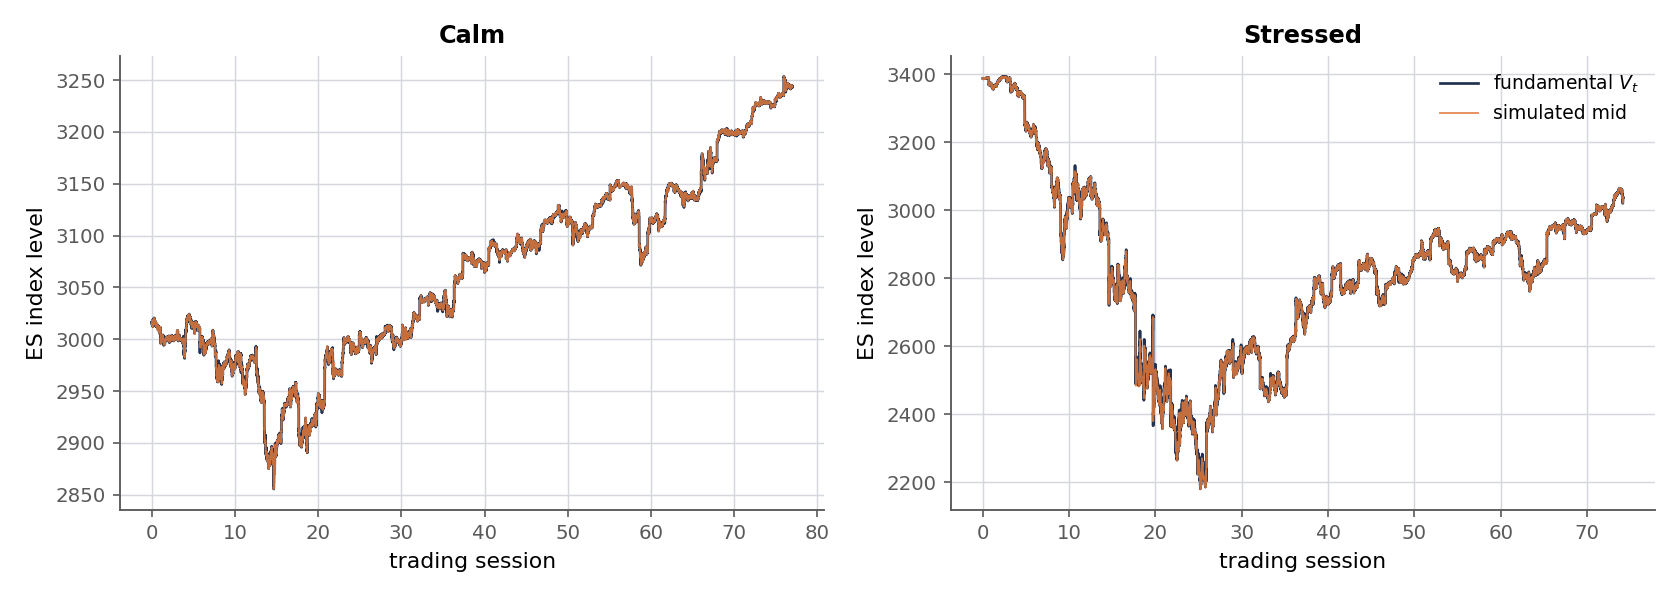
\includegraphics[width=\textwidth]{Figures/E_fv_vs_mid.png}
  \caption{\textbf{Fundamental versus simulated mid.} Empirical fundamental $V_t$ and the simulated mid
  with the clearing tier active, calm and stressed.}
  \label{fig:res-fv}
\end{figure}

\paragraph{Capital Ratios and Clearing Members.} In the stressed regime, members are pushed towards the capital-adequacy ratio of 8\% that they share. The BCMs occasionally breach and deleverage, and the NBCMs breach less often and freeze. NBCMs also sit with a higher capital ratio on average (Figure~\ref{fig:res-kappa}), but on the rare occasion where they do hit the floor and freeze, they are the only CM type that defaults. 

Each stressed seed produces an average $8.3$ client defaults (range $2$--$18$) and no defaults in calm. When the clients default, their CM seizes their IM and absorbs the remaining VM shortfall. The loss is generally contained at the CM and never reaches the default fund. In the rare case of NBCM default, 
the residual deficit it leaves --- on average
$\approx\$1.1$B --- is drawn up the waterfall: the defaulter's own default-fund contribution
($\approx\$0.11$B) and the CCP's skin-in-the-game ($\approx\$0.12$B) first, then the mutualised pooled
default fund ($\approx\$0.87$B). Against an average fund size of $\approx\$4.5$B in stress (and
$\approx\$6.3$B in calm) this draws about $19\%$ of the pooled fund.

\begin{figure}[H]\centering
  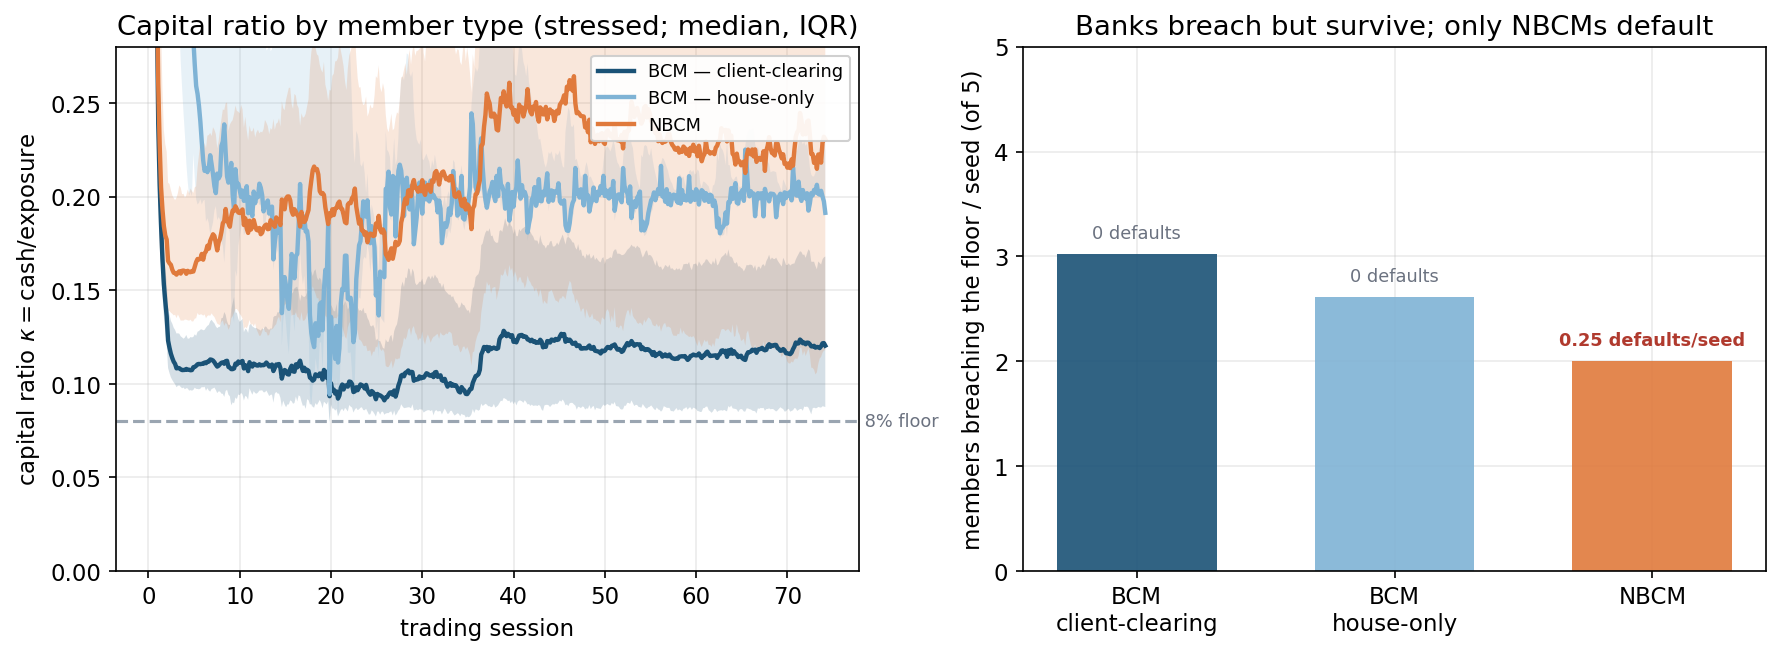
\includegraphics[width=\textwidth]{Figures/B_capital_ratio.png}
  \caption{\textbf{Clearing-member capital ratio $\kappa$.} Left: median $\kappa$ by member type over
  the stressed window (IQR band); the banks ride the $8\%$ floor (dashed) while the non-banks sit
  higher. Right: per-seed floor breaches and defaults by type --- banks breach but deleverage and
  survive, while the non-banks, unable to deleverage, are the only tier that defaults. In calm all
  members sit far above the floor.}
  \label{fig:res-kappa}
\end{figure}

\noindent This stylised result from the model stresses the importance for NBCMs to have an available external funding source that is reliable even in stressful market situations. The lack of an own book that can be liquidated to generate liquidity is a vulnerability for the NBCM, even when it freezes all client trading at a capital ratio of 8\%.

\paragraph{Margin is procyclical and clusters.} Posted margin sits at the anti-procyclicality floor of 4\% for the entirety of the calm period and the start of the stressed period, ramping up to a peak of $11.4\%$ in stressed, averaging at $7.7\%$ over the window (Figure~\ref{fig:res-im}), a result of the volatility sensitive VaR margining.

\begin{figure}[H]\centering
  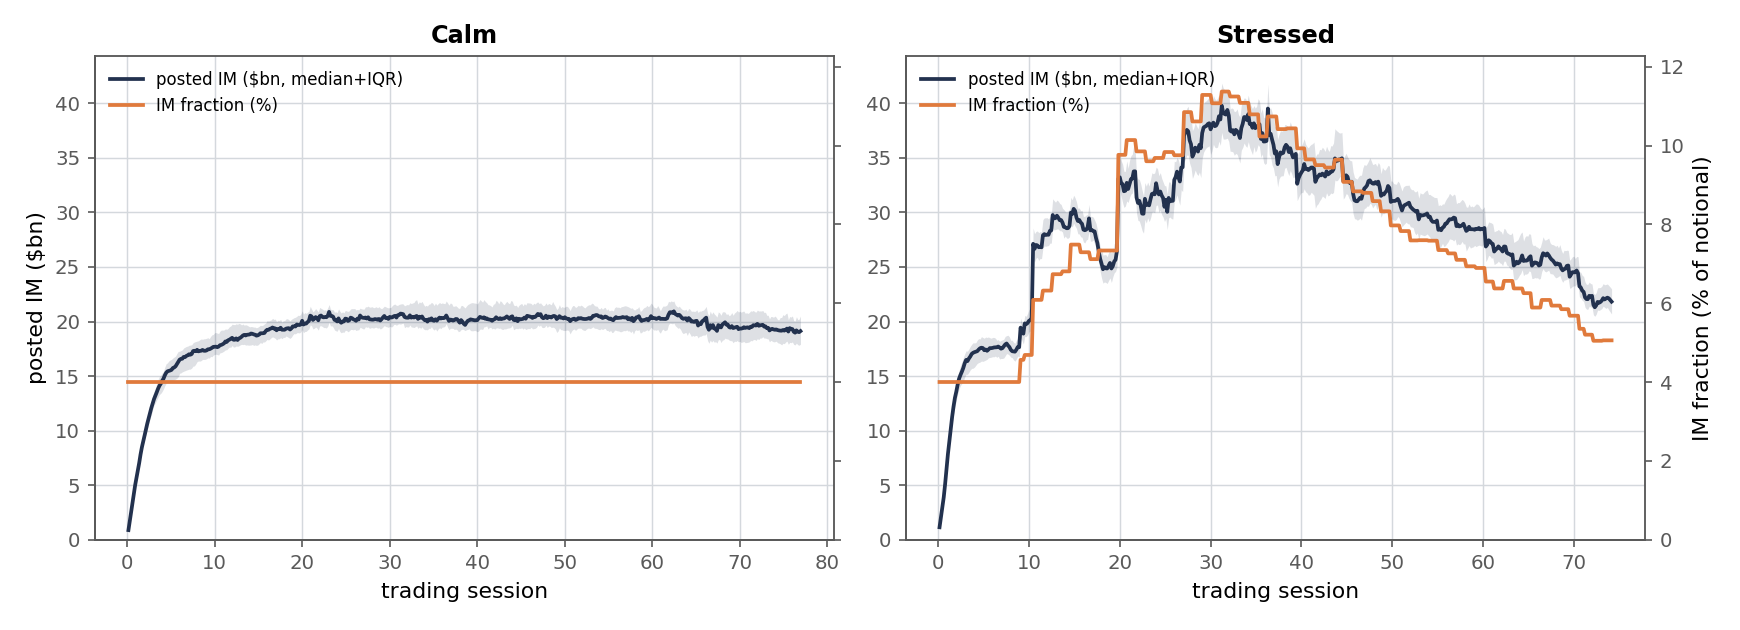
\includegraphics[width=\textwidth]{Figures/C_im_path.png}
  \caption{\textbf{Initial margin: dollar path and procyclical fraction.} Posted IM (left axis, median
  and IQR) and the charged fraction (right axis): flat at the $4\%$ floor in calm, ramping to $11.4\%$
  in stress.}
  \label{fig:res-im}
\end{figure}

\noindent Under stress, clients post roughly half of all initial margin (Figure~\ref{fig:res-imtype}). The client tier therefore has a large impact on collateral demand. We also see that FTs post the most amount of collateral, and MTs vary quite sharply in the collateral they post, a result of both higher margin requirements and increased trading in stressed markets due to their strategy and a persistent negative drawdown.

\begin{figure}[H]\centering
  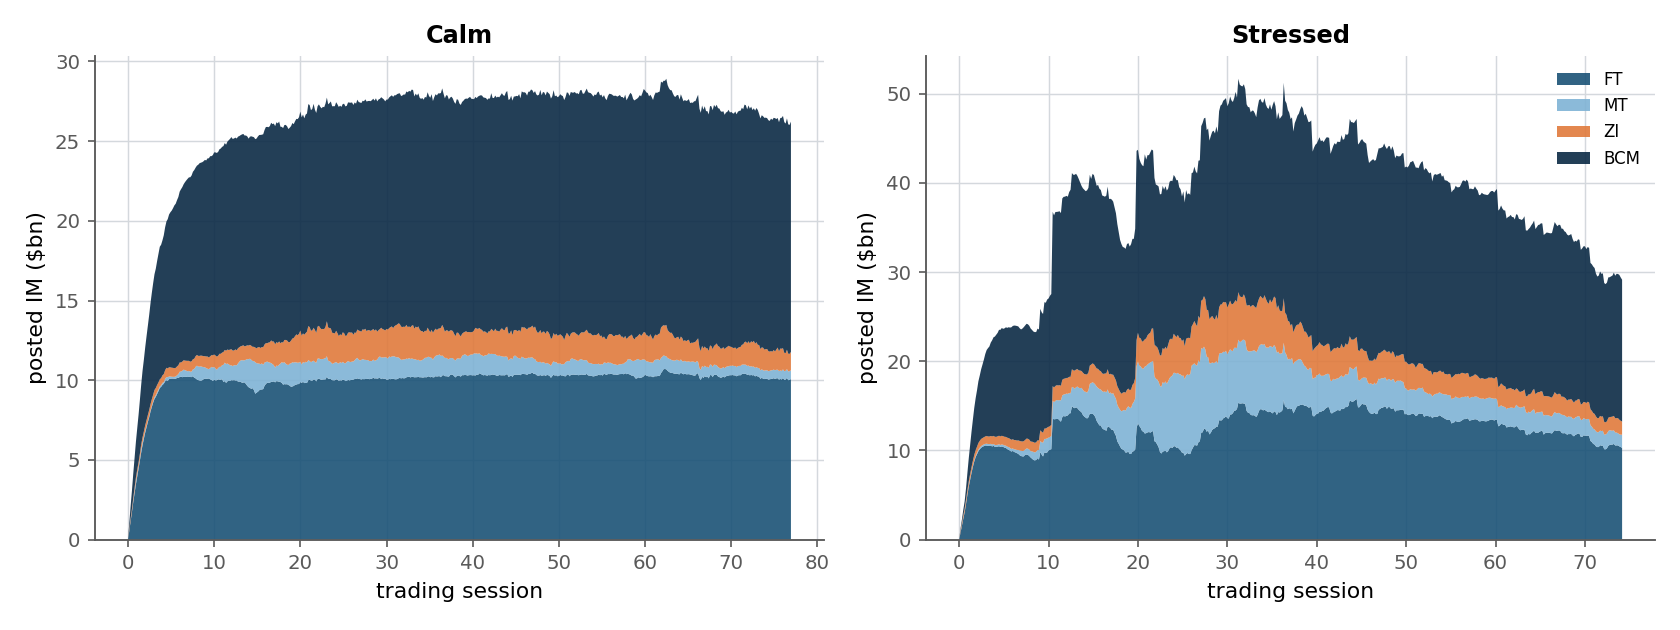
\includegraphics[width=\textwidth]{Figures/D_im_by_type.png}
  \caption{\textbf{Posted initial margin by participant type.} Fundamental, momentum and noise clients
  versus banking-member house margin; clients post about half of the total.}
  \label{fig:res-imtype}
\end{figure}

\noindent Looking at the arrival of margin calls, we see that they cluster over time, with bursts during stress (Figure~\ref{fig:res-mc}), emerging from the replicated volatility clustering in the model. This leaves CMs and clients prone to destabilising margin spikes during periods of extreme stress. 

\begin{figure}[H]
  \centering
  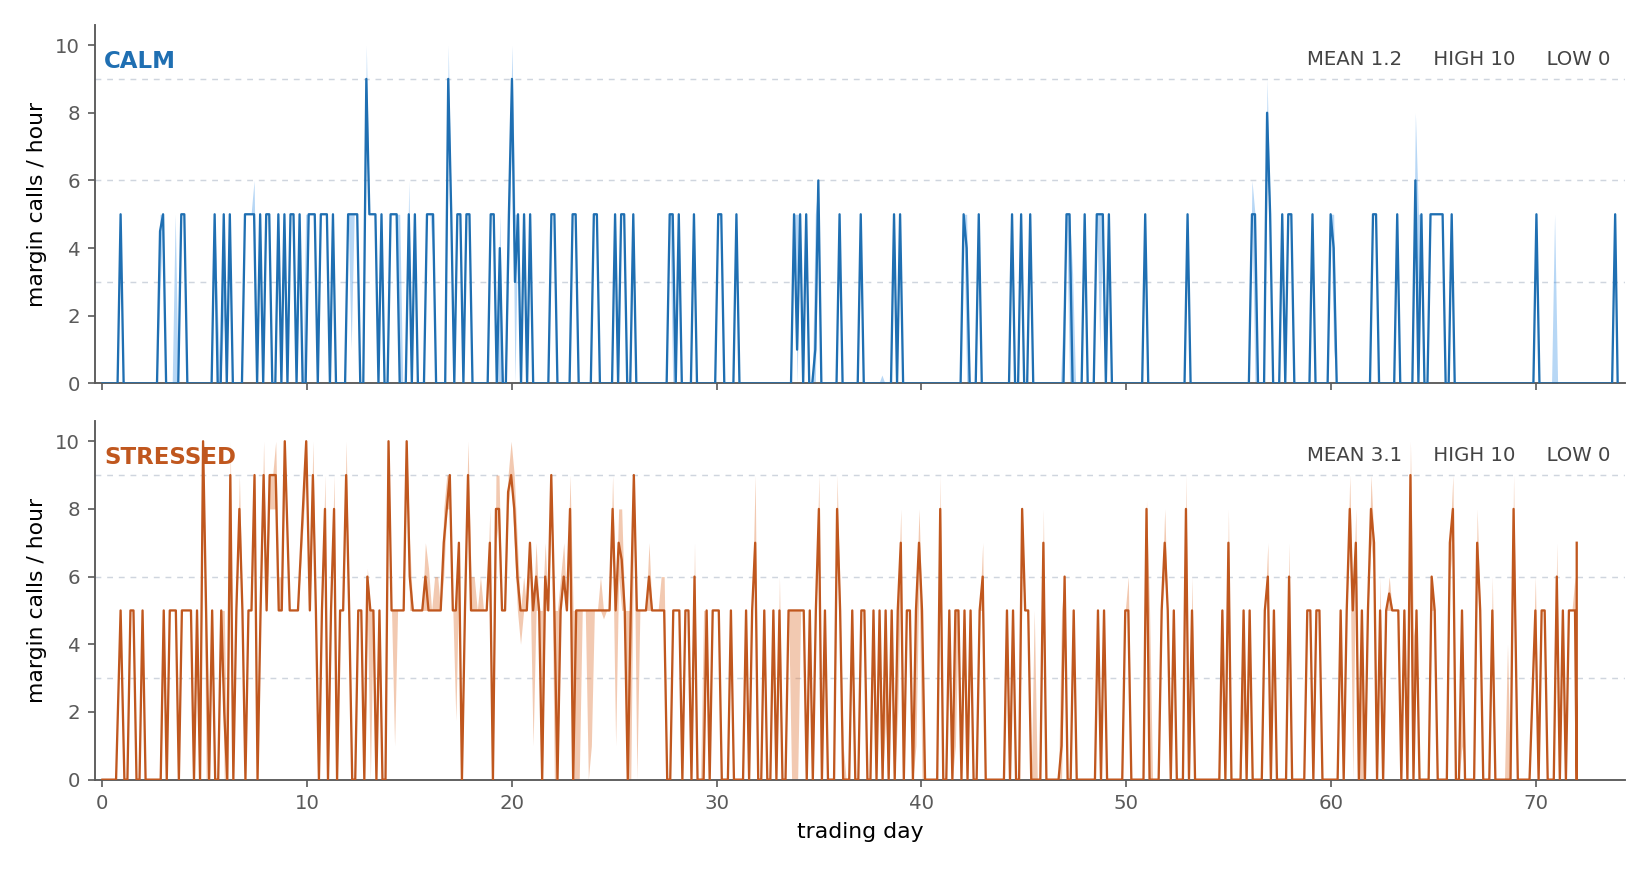
\includegraphics[width=\textwidth]{Figures/F_margin_call_clustering.png}
  \caption{\textbf{Margin-call clustering.} Margin calls per hour, calm (top) versus stressed (bottom); hours exceeding three calls are shaded. The wide, sustained bands under stress (54\% of hours) versus scattered spikes in calm (24\%) show the calls arriving in clusters rather than at random.
}
  \label{fig:res-mc}
\end{figure}

\section{Margin Procyclicality}\label{sec:resh1}

The model is then applied to look at margining practices -- volatile reactive margining is compared to flat and constant margins at different levels. Volatility sensitive margining is procyclical by construction, demanding collateral in stressful times where liquidity is hardest to raise \citep{brunnermeier_pedersen_2009,glasserman_wu_2018}. An anti-procyclicality (APC) buffer is standard practice, it asks for higher margins in calm times such that margins don't spike as much in stress. For the standard model, this was set at 4\% as covered in Section~\ref{sec:clearing-margin}. Here we look at a simple and explicit trade-off, we replace the reactive VaR margining with flat and constant margining at 3 levels -- 4\%, 8\%, and 12\%. 

The low level at 4\% is a plausible lower bound for an asset as liquid as ES futures, and is the current APC buffer in the standard model. The intermediate 8\% is close to the average margin the reactive VaR model asks for in stress times, and the high level at 12\% covers the peak of margin asked for by the model in stress. Each of these, alongside the reactive VaR margining, is run over 150 seeds and evaluated based on client defaults, member defaults, how far losses travel up the waterfall and how much it costs to post these levels of collateral.

The default fund (DF) of the standard model had to be adjusted to account for this construction. The standard model uses a Stressed-loss-over-margin to size the DF, but for the high flat IMs this often led to the DF collapsing to zero. The experiment therefore substitutes a fixed default fund, sized at $10\%$ of the two largest
members' positions (a cover-2 principle) at $\approx\$12$--$14$B --- comparable to CME Clear's --- and
applies it to both the flat and reactive arm, so that differences reflect the
margin rule alone.\\

\noindent From the results, we see that higher margin does not remove default risk but rather relocates it. As margin rises from a fixed 4\% to 12\%, client defaults fall but member defaults rise (Table~\ref{tab:res-h1}). The proportion of times the default fund is reached also rises. This happens due to a concentration of losses -- client failures become rare but also larger, falling on the member tier. The mechanism behind these is discussed further in Subsection~\ref{sec:res-mech}. While the client default decline is significant, member defaults and mutualisation are rare events and hence noisy and not statistically significant. They are, however, significant in their direction and robust to different clearing constants such as a different house capital ratio floor, default fund level and CCP recovery amount. 

\begin{table}[H]
\centering\small
\caption{\textbf{H1 --- margin regimes (stressed, 150 seeds).} Client defaults mean (sd); other columns mean
across seeds; IM in \$B; run under the ODD fixed default fund ($\approx\$12$--$14$B across arms) so the
mutualised layer is comparable. The \emph{flat ladder} reads the trade-off top-to-bottom: as the standing
margin rises, cost rises and client defaults fall, but loss climbs the waterfall (member defaults and
mutualisation rise). \emph{Reactive} (set off below) holds the flat-$4\%$ standing cost while matching
flat-$8\%$'s stress protection (its lower risk-metric means are within seed noise) --- its cost is the
stress-time \emph{peak}.}
\label{tab:res-h1}
\begin{tabular}{l cc c cc}
\toprule
 & \multicolumn{2}{c}{Cost (\$B)} & Clients & \multicolumn{2}{c}{Loss up the waterfall} \\
\cmidrule(lr){2-3}\cmidrule(lr){5-6}
Margin regime & calm & peak & client def. & member def. & reach fund \\
\midrule
Flat $4\%$    & $18.1$ & $18.6$ & $14.8\ (4.8)$ & $0.01$ & $\phantom{0}1\%$  \\
Flat $8\%$    & $31.7$ & $33.8$ & $11.1\ (4.7)$ & $0.35$ & $30\%$ \\
Flat $12\%$   & $42.3$ & $46.3$ & $\phantom{0}6.9\ (4.4)$ & $0.55$ & $42\%$ \\
\midrule
Reactive ($4\!\to\!11.4\%$) & $18.1$ & $38.5$ & $10.1\ (4.3)$ & $0.33$ & $25\%$ \\
\bottomrule
\end{tabular}
\end{table}

The attractiveness of the VaR reactive margin can be easily seen, it offers performance on risk-metrics just as well if not better than the flat 8\% margin. At the same time, it asks for a significantly lower amount of margin in calm periods and not much higher in stress (Figure~\ref{fig:res-h1}). 

\begin{figure}[H]
  \centering
  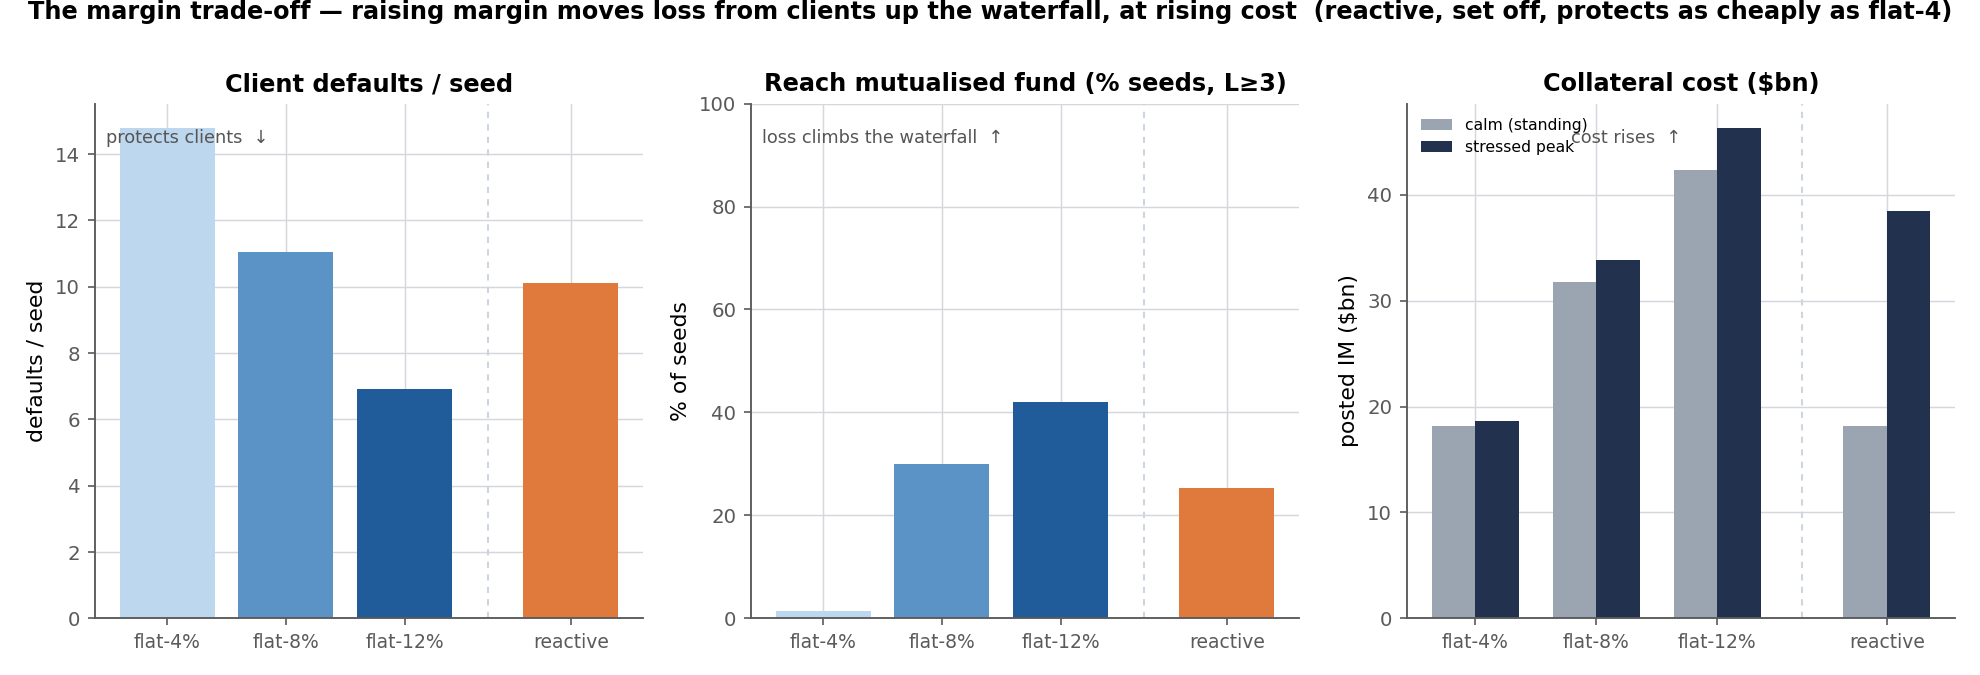
\includegraphics[width=\textwidth]{Figures/H1_margin.png}
  \caption{\textbf{H1 --- the margin trade-off.} Each panel is one outcome across the margin regimes; the
  flat ladder (light to dark) is monotonic and reactive is set off (after the dashed line) and highlighted.
  Raising the flat margin protects clients (client defaults fall, left) but pushes loss up the waterfall
  (mutualisation rises, centre) at rising standing cost (right). Reactive protects about as cheaply as
  flat-$4\%$ in calm while matching flat-$8\%$'s stress protection, paying only a stress-time peak (dark bar,
  right).}
  \label{fig:res-h1}
\end{figure}

\subsection{Mechanism: loss relocation}\label{sec:res-mech}

The relocation of defaults from clients to members as flat IM increases offers an interesting avenue for further analysis. This relocation appears to stem from CM freezes -- CMs that breach their capital adequacy floor (CAR) stop clearing, freezing their clients. The position of these clients then accumulates VM transfers due to negative returns. With higher margins, more cash is taken as margin and hence members breach their CAR earlier in the crash, but at the same time, this turns into a trap. Due to the early freeze, clients holding onto a large position cannot liquidate it and default as the market falls. Despite the median of defaulted positions being lower for higher flat margins, the tail of positions on default is a lot higher (Figure~\ref{fig:mech-position}). The member then assumes this large position that it must liquidate onto a falling market, and the losses on this overwhelm especially the NBCMs causing them to default. 

\begin{figure}[H]\centering
  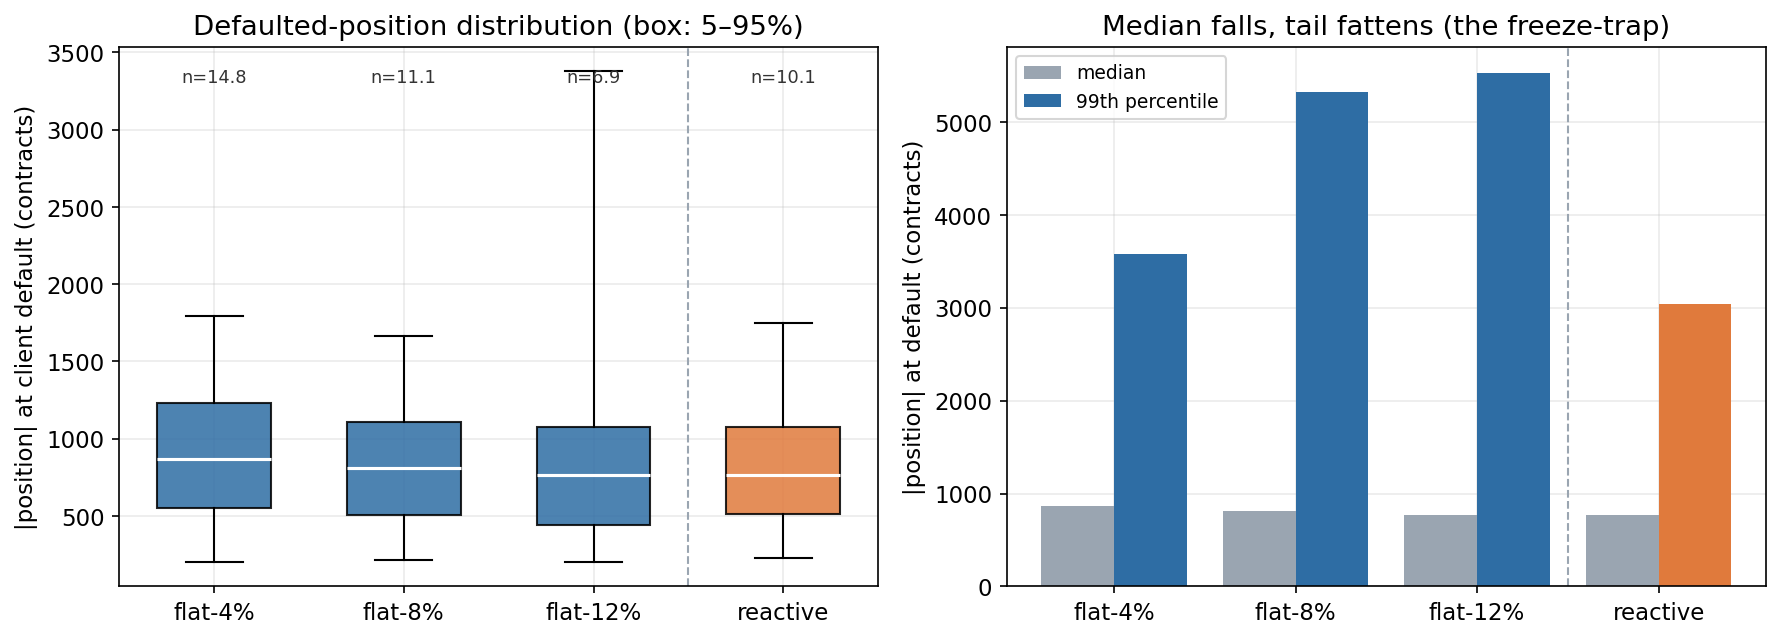
\includegraphics[width=\textwidth]{Figures/mech_position.png}
  \caption{\textbf{The freeze-trap.} Distribution of $|$position$|$ at client default by margin regime
  (left; box spans $5$--$95\%$, $n=$ defaults per seed) and the median versus the $99$th percentile
  (right). Higher flat margin yields fewer, smaller-median defaults but a fatter tail; reactive keeps
  the tail thin.}
  \label{fig:mech-position}
\end{figure}

\noindent This highlights the vulnerability these clients face by having only a single clearing connection at the mode \citep{ofr_2026}. If a CM facing capital or liquidity constraints decides to freeze offering clearing services to its clients, the clients are left holding onto a possible unwanted position that by regulation must be centrally cleared. At the same time, this is also a consequence of the simplified model design. In reality, an inability to liquidate is not an absolute, but in stressed market situations, porting and finding new members would prove to be difficult. \cite{acosta_smith_2018} also show that capital ratio requirements did leave members less willing to provide clearing services.  


\section{A Synthetic Path Alternative}\label{sec:res-synth}

So far, the results replay a historical period, using the empirical mid price as a Fundamental Value. This creates a natural limitation for this model - it can only be simulated over one path. This section provides an alternative, switching out the FV for a stochastic and synthetic series that reproduces the same stylised facts seen in the stressed period. The parameters of the synthetic FV are then calibrated jointly with agent parameters to reproduce stressed empirical moments, with the calibration yielding a fit in stress near identical to the empirical path, with moments such as volatility clustering being better reproduced (Section~\ref{sec:cal-synth}). The simulation is then run on 80 seeds, yielding 80 different paths for the Fundamental Value, and hence also for the simulated mid. The drift of these paths is similar to the COVID stressed window, but the stochastic runs yield both less and more extreme paths (Figure~\ref{fig:synth-paths}), which makes it well suited to studying CCP resilience across many stress scenarios.

\begin{figure}[H]
  \centering
  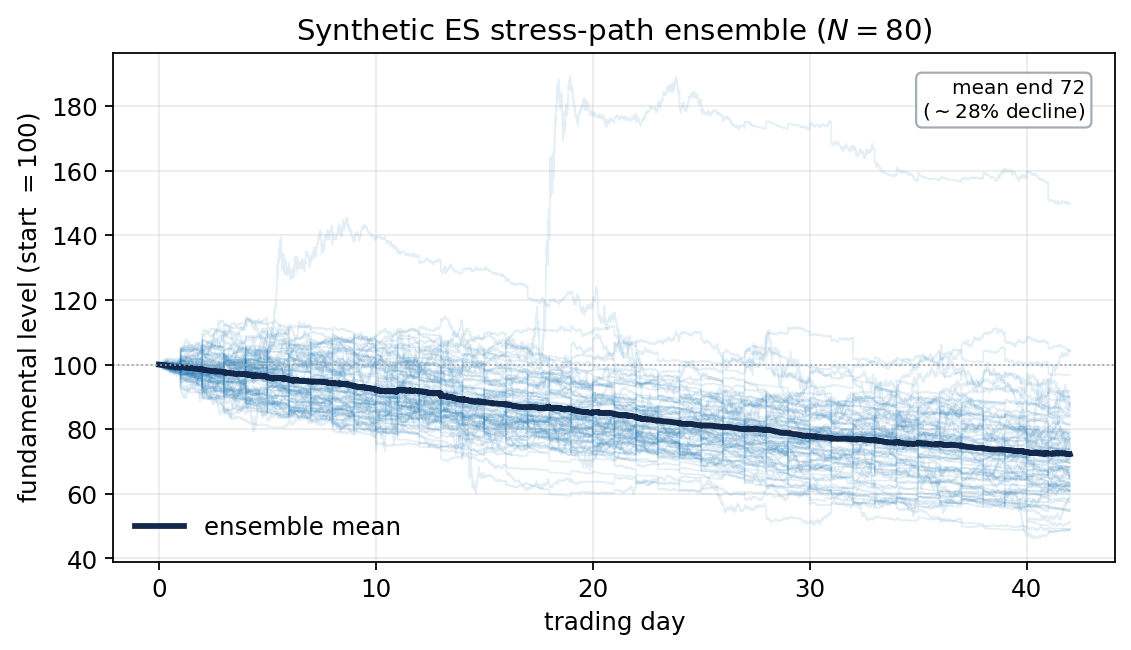
\includegraphics[width=0.72\textwidth]{Figures/synth_paths.png}
  \caption{\textbf{Synthetic two-factor-SV stress-path ensemble.} $N=80$ independent synthetic ES fundamental
  paths (thin) with the ensemble mean (bold), drifting down at the stressed-window rate.}
  \label{fig:synth-paths}
\end{figure}

\paragraph{A tail within a tail.} A point to note is that these paths are already based on a stressed environment, one that would form the tail of any normal distribution. The median path here is hence already a tail path. We see that despite this, for the median path, there are only 3 client defaults, no member defaults, and the default fund is never drawn (Table~\ref{tab:synth-clearing}). Across 80 such extreme paths, only 14 reach the mutualised default fund in this stylised model. 

\begin{table}[H]
\centering\small
\caption{\textbf{Clearing outcomes across the $N{=}80$ synthetic stressed ensemble} (reactive margining,
$42$-day paths). Posted initial margin in \$B; the waterfall levels L1--L5 follow the model's five-level
default waterfall (L3 the mutualised default fund, L4 surviving-member loss-sharing, L5 CCP capital).}
\label{tab:synth-clearing}
\begin{tabular}{lccc}
\toprule
 & Median path & Ensemble mean & Worst path \\
\midrule
Client defaults          & $3$    & $7.8$  & $68$   \\
Member defaults          & $0$    & $1.0$  & $15$   \\
Peak posted IM (\$B)     & $43.5$ & $44.7$ & $80.8$ \\
Deepest waterfall level  & $0$    & ---    & $5$    \\
\midrule
\multicolumn{4}{l}{\footnotesize $14/80$ paths reach the mutualised default fund (L$\geq3$); $8$ reach
member loss-sharing (L4); $3$ reach CCP cash (L5).}\\
\bottomrule
\end{tabular}
\end{table}

\paragraph{Volatility and drawdowns.} Looking at the paths by realised volatility, the first two-thirds are benign. There are around 3 client defaults per path, no member defaults and the default fund isn't breached. The defaults and stress are concentrated in the bottom third. Interestingly, the median drawdown of the paths that breach the DF is $29\%$, lower than the median $35\%$ of the paths that never breach. Furthermore, the clearing outcomes carry a robust rank correlation with realised volatility (Spearman
$\rho\approx0.5$, $p<0.001$, $n=80$) but none with the net drawdown. This can perhaps be explained by the margin mechanism, VM simply transfers from one member to another and is redistributed. IM, on the other hand, drains the balance of all members (Figure~\ref{fig:synth-clearing}). This rises with volatility, and offers an insight into just how draining IM can be with VaR margin models. 


\begin{figure}[H]
  \centering
  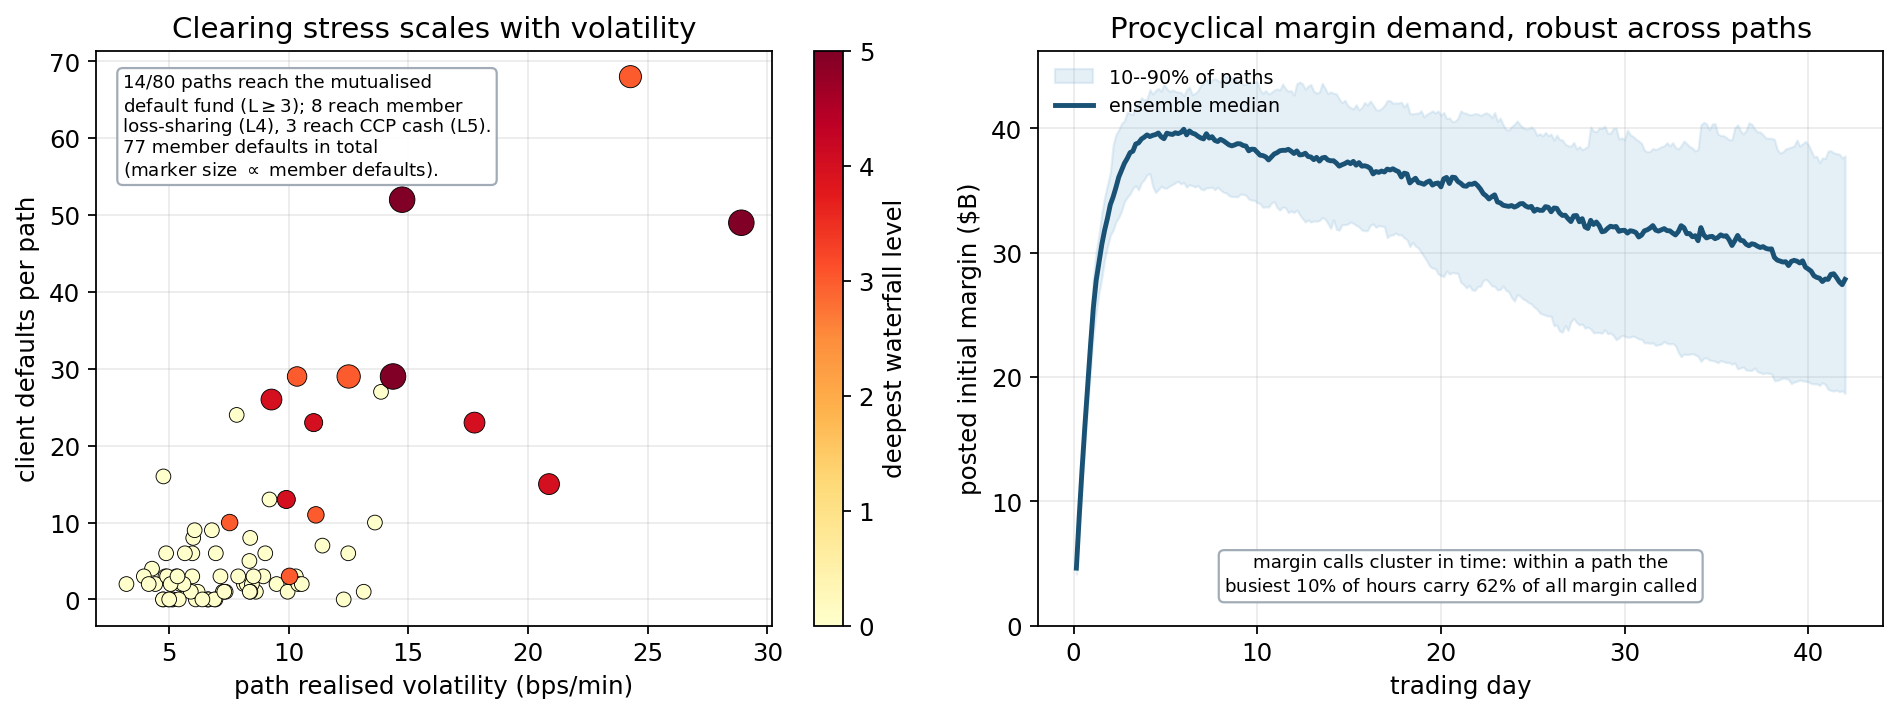
\includegraphics[width=\textwidth]{Figures/synth_clearing.png}
  \caption{\textbf{Clearing on the synthetic stressed ensemble.} Left: per-path clearing stress (client
  defaults) against the path's realised volatility, coloured by the deepest waterfall level reached and sized
  by member defaults. Right: posted initial margin over the window (ensemble median and $10$--$90\%$ band) --- the
  procyclical ramp is consistent across all $80$ paths, while within a path the calls themselves cluster in
  time.}
  \label{fig:synth-clearing}
\end{figure}

Overall, the member tier can absorb defaults across the median stressed paths. The extreme paths, however, do push the CCP to its limits, exhausting default funds and tapping into member cash reserves. While the model is a definite simplification, and some results may emerge as a consequence of model design over being an accurate representation of society, its ability to simulate outcomes across various paths, studying the effects of changes in various parameters and CCP recovery practices offers a definite benefit.  